\chapter{Local strategies are pretty good at computing boolean properties of quantum sequences} \label{ch:qseq}

Suppose there are two known quantum states, $\ket{\psi}$ and $\ket{\phi}$, and a learner receives a sequence of the form
\begin{equation}
    \ket{\psi}\ket{\phi}\ket{\psi}\cdots\ket{\psi} .
\end{equation}
While each position is known to be either $\ket{\psi}$ or $\ket{\phi}$, the identity of each state is unknown. 
Can one determine whether the number of $\ket{\psi}$ states exceeds the number of $\ket{\phi}$ states, or whether the total number of $\ket{\psi}$ states is even? 
These examples highlight a basic task: learning coarse-grained properties of a quantum sequence without determining the sequence itself.

We study this problem in two contrasting resource regimes. 
In the \emph{full-memory} setting the entire (finite) sequence may be stored so that an optimal joint measurement can be performed upon receiving all of the states. 
In the \emph{memoryless} setting, neither quantum nor classical memory is available and each state must be measured immediately, using only predetermined local measurements. 
This work investigates which Boolean properties can still be learned optimally under such stringent memory constraints.

Motivated by this, we initiate a study of learning Boolean properties of quantum sequences. 
In a classical information-processing/computation setup, data are represented by bit strings, and computing Boolean functions of these strings, such as the $\mathsf{XOR}$ is elementary; the main challenges lie instead in algorithmic efficiency and robustness of protocols. 
In the quantum setting, by contrast, computing even a simple function becomes non-trivial when no classical description of the data is available. 
We consider which properties can be optimally learned using memoryless measurement strategies, and which fundamentally require joint measurements across the sequence. 
The paradigm we focus on is minimum-error, where the learner might obtain an incorrect value for the property of the sequence and their goal is to minimize this error, and we completely characterize the Boolean functions for which fixed local measurements are optimal.

%------------------------------------------------------------------------------%
\section{Problem Formulation and Main Results} \label{sec:ch5_qseq-main}
%------------------------------------------------------------------------------%
In this section we formulate our problem as a task of quantum state discrimination and present the main results. 
%The section ends with a short guide to the structure of the paper.

\subsection{Problem Formulation}

In classical computing, data are modeled by bit strings. 
In our setting, we consider encoding the classical symbols 0 and 1 into two fixed, arbitrary non-orthogonal quantum states $\ket{\psi_0}$ and $\ket{\psi_1}$. 
This induces a map from an $n$-bit string $x \in \bit^n$ to a product quantum state of length $n$: 
\begin{equation} 
    x = x_1 x_2 \cdots x_n \in \bit^n \longmapsto  \ket{\psi_x} := \ket{\psi_{x_1}} \otimes \ket{\psi_{x_2}} \cdots \otimes \ket{\psi_{x_n}}.
\end{equation} 
Any Boolean property of the resulting quantum sequence can be described by a Boolean function $f:\{0,1\}^n \to \{0,1\}$. 
Learning this property, equivalently, determining the value of $f(x)$ does not require full identification of the underlying string $x$. 
Rather, it suffices to discriminate between the two sets of quantum sequences corresponding to inputs for which $f(x)=0$ and for which $f(x)=1$. 
Thus, given an unknown quantum sequence $\ket{\psi_{x}}$, the task is to decide whether the classical label $x$ belongs to $S_0$ or $S_1$, where $S_0 = f^{-1}(0)$ and $S_1 = f^{-1}(1)$ are the pre-images of 0 and 1 respectively. Using standard arguments, without loss of generality we can consider $\ket{\psi_0}$ and $\ket{\psi_1}$ to be qubit states with a nonnegative inner product \cite[Section~3.1]{barnett2008discrimination}.
Furthermore, since orthogonal and identical states represent trivial discrimination cases, we restrict the inner product to the open interval $\braket{\psi_0}{\psi_1}=s \in (0,1)$.

To learn the property\footnote{Henceforth we will use the terms ``property'' and ``function'' interchangeably.} $f$, the learner must discriminate between two mixed quantum states $\sigma_0$ and $\sigma_1$ where $\sigma_i$ is the density matrix obtained by mixing the states $\left\{\ketbra{\psi_x}{\psi_x} : f(x) = i\right\}$. 
Assuming a uniform prior over the input strings in $\{0,1\}^n$, these mixed states can be written as
\begin{equation}
    \label{eq:ch5_qseq-states}
    \sigma_0 = \frac{1}{|S_0|} \sum_{x \in S_0} \ketbra{\psi_x}{\psi_x} \quad \text{and} \quad \sigma_1 = \frac{1}{|S_1|} \sum_{x \in S_1} \ketbra{\psi_x}{\psi_x},
\end{equation}
which occur with prior probabilities $p_0 = |S_0|/2^n$ and $p_1 = |S_1|/2^n$. 
We refer to the resulting ensemble 
\begin{equation}
    \label{eq:ch5_qseq-boolean-ensemble}
    \mathcal{E} = \{(p_0,\sigma_0),(p_1,\sigma_1)\}
\end{equation} 
as the Boolean ensemble. 
In this work we consider the \emph{minimum-error} evaluation of the function $f$, where the learner performs a measurement on the unknown quantum state $\ket{\psi_x}$ to infer the value of $f(x)$, seeking to minimize the probability of error. 
Operationally, this corresponds to discriminating between $\sigma_0$ and $\sigma_1$ using a two-outcome POVM \\ $\mathcal{M} = \{ M_0, M_1 \}$, where the outcome $i$ is interpreted as the guess $f(x)=i$. 
Conditioned on the state being $\sigma_i$, the probability of correct guess is $\inner{M_i}{\sigma_i}$. 
The optimal success probability is obtained by maximizing the average probability of a correct decision over all such POVMs:
\begin{equation} 
    \label{eq:ch5_qseq-qsd}
    \max \left\{ 
        p_0 \inner{M_0}{\sigma_0} + p_1 \inner{M_1}{\sigma_1} : M_0 + M_1 = \I, M_0, M_1 \geq 0 
    \right\}.
\end{equation} 
This is a semidefinite program and generalizes to discrimination among any finite ensemble of quantum states. 
Since this is a case of two states, the optimal minimum-error success probability is given by the Helstrom bound \cite{helstrom1969quantum,holevo1976investigations}
\begin{equation} 
    \label{eq:tracenorm}
    \frac{1}{2} + \frac{1}{2} \| p_0 \sigma_0 - p_1 \sigma_1 \|_{1}
\end{equation} 
where $\| X \|_{1} = \tr\left(\sqrt{X^*X}\right)$ is the trace norm. 

An optimal POVM achieving the maximum success probability may require a joint measurement acting on the entire $n$-qubit state $\ket{\psi_x}$, which is technologically challenging \cite{lvovsky2009optical,ma2021one,conlon2023approaching}. 
A feasible alternative is a local measurement strategy, in which each state is measured individually. 
Such a strategy effectively extracts classical information from each subsystem and uses it to infer the value of $f(x)$. 
In this work, we focus on a simple type of strategy:
a fixed local strategy that applies a predetermined measurement to each subsystem, independent of all of the previous outcomes, thus requiring neither classical nor quantum memory. 
A natural fixed local strategy to consider is the one which aims to optimally distinguish between $\ket{\psi_0}$ and $\ket{\psi_1}$ at each position. 
Thus, given any Boolean function $f$, this strategy learns each bit optimally, constructs a guess for the encoded string, and evaluates $f(x)$. This can also be seen as a \emph{non-adaptive greedy} strategy\footnote{Note, however, that this notion of greediness does not always yield local measurements that are optimal for computing the overall function value. This is more evident for unbalanced functions, such as AND and OR.}.
One might be tempted to think that this naive and simple strategy would perform rather poorly when compared with a global measurement. 
Our first result shows that, remarkably, this strategy performs rather well---but first we establish some notation.
\begin{definition}
    Given a positive integer $n$, a function $f : \bit^n \to \bit$, the two encoding qubit states $\ket{\psi_0}$ and $\ket{\psi_1}$ with inner product $s = \braket{\psi_0}{\psi_1}$, then the optimal success probability of learning the function $f$ using a strategy \emph{strat} when each $x \in \bit^n$ is chosen uniformly at random is denoted by $P(n,f,s,\mathrm{strat})$.
\end{definition}
Throughout this paper, we write $\greedy$ and $\glo$ to denote the fixed local (greedy) strategy and a globally optimal strategy, respectively.  

\subsection{Main results} 

We now state our first main result which establishes an universal performance guarantee for the greedy strategy.
\begin{theorem}
    \label{thm:ch5_qseq-PGM}
    For all Boolean functions $f$, positive integers $n$, and $s \in (0,1)$, the performance of the greedy strategy can be bounded below by the following relation
    \begin{equation}
        (P(n,f,s,\glo))^2 \leq P(n,f,s,\greedy).
    \end{equation}
\end{theorem}

The proof consists in showing that the greedy strategy is implemented by the pretty good measurement (PGM) \cite{hausladen1994pretty} for discriminating the Boolean ensemble $\mathcal{E} = \{(p_0, \sigma_0), (p_1, \sigma_1)\}$. 
The bound then follows from Barnum and Knill's theorem~\cite{barnum2002reversing,watrous2018theory}. 
This is presented in Section~\ref{sec:easy-proofs}.

This raises a natural question: for which Boolean functions does the greedy strategy actually achieve the global optimum? 
The next result identifies a class of functions that satisfies this.

\begin{restatable}[Sufficiency]{theorem}{sufficient}
    \label{thm:ch5_qseq-sufficient}
    The greedy strategy is globally optimal, that is 
    \begin{equation}
        P(n,f,s,\greedy)=P(n,f,s,\glo)
    \end{equation} 
    for all Boolean functions of the form 
    \begin{equation}
        \label{eq:ch5_qseq-affine}
        f(x_1,\dots,x_n) = b_0 \oplus b_1 x_1 \oplus b_2 x_2 \oplus \cdots \oplus b_n x_n,
    \end{equation}
    where $b_0, b_1, \ldots, b_n \in \{0, 1\}$, for all $s \in (0,1)$.
\end{restatable}

The functions of the form in Eq.~\eqref{eq:ch5_qseq-affine} are called \emph{affine Boolean functions}. 
For affine functions, both the globally optimal success probability (via the Helstrom bound) and the greedy success probability can be computed in closed form. 
A direct calculation using properties of the trace norm shows that they are equal for all $s \in (0,1)$. 
See Section~\ref{sec:ch5_qseq-easy-proofs} for details.

Our final result shows that this class is essentially the only one for which the greedy strategy is optimal, establishing a converse to Eq.~\eqref{thm:ch5_qseq-sufficient}.

\begin{restatable}[Necessity]{theorem}{necessity}
    \label{thm:ch5_qseq-necessary}
    For learning a Boolean function $f:\{0,1\}^n \to \{0,1\}$, if the greedy strategy is globally optimal, then $f$ must be an affine Boolean function of the form in Eq.~\eqref{eq:ch5_qseq-affine} for all but finitely many values of $s \in (0,1)$.
\end{restatable}

\begin{restatable}[Sufficiency]{theorem}{sufficient}
    \label{thm:ch5_qseq-sufficient}
    Suppose $f:\{0,1\}^n \to \{0,1\}$ is affine Boolean. 
    Then greedy = global, for $s \in (0,1)$.
\end{restatable}

\begin{restatable}[Necessity]{theorem}{necessity}
    \label{thm:ch5_qseq-necessity_v1}
    Suppose $f:\{0,1\}^n \to \{0,1\}$ is not affine Boolean. 
    Then greedy < global, for all but possibly finitely many values of $s \in (0,1)$.
\end{restatable}

\begin{restatable}[Necessity]{theorem}{necessity}
    \label{thm:ch5_qseq-necessary_v2}
    For all but finitely many values of $s \in (0,1)$, if the greedy strategy is globally optimal for learning a Boolean function $f:\{0,1\}^n \to \{0,1\}$, then $f$ must be an affine Boolean function of the form in Eq.~\eqref{eq:affine}.
\end{restatable}

Together, Theorems~\ref{thm:ch5_qseq-sufficient} and~\ref{thm:ch5_qseq-necessary} provide a complete characterization: affine Boolean functions are precisely those for which memoryless measurement strategies suffice for optimal learning. 
Note that Theorem~\ref{thm:ch5_qseq-necessary} holds for all $s \in (0,1)$ except possibly for a finite set, hence for all but a set of measure zero. 
The proof is presented in Section \ref{sec:ch5_qseq-necessary}. 
This is followed by discussing the conclusions (Section \ref{sec:ch5_qseq-discussion}). 

Section~\ref{sec:ch5_qseq-non_affine_examples} briefly discusses the performance of the greedy strategy for some non-affine functions. 
We consider the $\mathsf{AND}$ and $\mathsf{MAJ}$ (majority) functions as representative non-affine examples. 
The former is highly unbalanced ($|S_0|=2^n-1, |S_1|=1)$, while the latter is balanced ($|S_0|=|S_1|)$. 
In both cases, globally optimal strategies outperform the greedy strategy, as illustrated by numerical results for small sequence lengths ($3\le n\le 9$). 
Their asymptotic behavior, however, differs: for $\mathsf{AND}$, both the greedy and global strategies achieve perfect success as $n\to\infty$, whereas for $\mathsf{MAJ}$, the greedy strategy remains bounded away from unity in this limit.

%%%%%%%%%%%%%%%%%%%%%%%%%%%%%%%%%%%%%%%%%%%%%%%%%%%%%%%%%%%%%%%%%%%%%%%%%%%%%%%%%%%%%%%%%%%%%%%%%%%%%%%%%%%%%%%%%%%%%%%%%%%%%%%%%%

\section{Proofs of Theorems~\ref{thm:ch5_qseq-PGM} and~\ref{thm:ch5_qseq-sufficient}: Performance of the Greedy Strategy}\label{sec:ch5_qseq-easy_proofs}

\amnote{Move this to the introduction}

The \emph{pretty good measurement} (PGM), introduced by Hausladen and Wootters~\cite{hausladen1994pretty} and further analyzed by Barnum and Knill~\cite{barnum2002reversing}, provides a computationally tractable measurement strategy for quantum state discrimination. 
Given an ensemble $\{(p_i, \rho_i)\}_{i=1}^n$, the PGM is defined by the measurement operators
\begin{equation}
    \label{eq:ch5_qseq-pgm_operators}
    M_i^{\text{PGM}} = \rho_{\text{avg}}^{-1/2} (p_i \rho_i) \rho_{\text{avg}}^{-1/2},
\end{equation}
where $\rho_{\text{avg}} = \sum_{i=1}^n p_i \rho_i$ and $\rho_{\text{avg}}^{-1/2}$ denotes its Moore-Penrose pseudo-inverse. These operators form a valid POVM.

Barnum and Knill~\cite{barnum2002reversing} gave the following bound on the performance of the PGM.

\begin{theorem}[Barnum-Knill Inequality \cite{barnum2002reversing}]
    \label{thm:ch5_qseq-barnum-knill}
    Let $P_{\text{opt}}$ denote the optimal success probability and $P_{\text{PGM}}$ denote the success probability achieved by the pretty good measurement for discriminating an ensemble $\{(p_i, \rho_i)\}_{i=1}^n$. Then
    \begin{equation}
        P_{\text{opt}}^2 \leq P_{\text{PGM}} \leq P_{\text{opt}}.
    \end{equation}
\end{theorem} 

This bound ensures that the PGM always achieves a success probability at least as large as the square of the optimal probability, guaranteeing near-optimal performance. 
Moreover, in many cases of interest, the PGM is exactly optimal \cite{mochon2006family,dalla2015optimality,eldar2001quantum}.

\subsection{The Greedy Strategy}

Let $\mathcal{M} = \{M_0, M_1\}$ be an optimal POVM for discriminating the ensemble \\ $\{(1/2, \ket{\psi_0}), (1/2, \ket{\psi_1})\}$ on a single qubit, where $M_0, M_1 \in \Pos(\C^2)$ satisfying $M_0 + M_1 = \I$. 
Since $\ket{\psi_0}$ and $\ket{\psi_1}$ appear with equal probabilities, the PGM is optimal for this single-qubit discrimination problem~\cite{hausladen1994pretty}, with
\begin{equation}
    M_i = \frac{1}{2} \rho^{-1/2} \op{\psi_i} \rho^{-1/2},
\end{equation}
for $i \in \{0, 1\}$ where $\rho = \frac{1}{2}\op{\psi_0} + \frac{1}{2}\op{\psi_1}$ is the average single-qubit state.

The greedy strategy operates as follows: 
measure each qubit of the sequence $\ket{\psi_x}$ independently using the POVM $\mathcal{M}$, obtaining outcome $y_i \in \{0,1\}$ for the $i$-th qubit, which gives us a classical string $y = y_1 \ldots y_n$. 
We then evaluate $f(y)$: if $y \in S_0$, we guess that the input was from $S_0$; if $y \in S_1$, we guess $S_1$.

The success probability of this strategy can be computed as follows. 
Given that the true input is $x$, the probability of obtaining outcome string $y$ through local measurements is
\begin{equation}
    \Pr[y \mid x] = \inner{M_y}{\op{\psi_x}} = \prod_{i=1}^n \inner{M_{y_i}}{\op{\psi_{x_i}}}.
\end{equation}
where $M_y = \bigotimes_{i=1}^n M_{y_i}$.

We succeed if $x$ and $y$ belong to the same set ($S_0$ or $S_1$). 
Averaging over the uniform distribution on inputs, the greedy success probability is
\begin{equation}
    \label{eq:ch5_qseq-local_success}
    \begin{aligned}
        P(n,f,s,\greedy) &= \sum_{x \in \{0,1\}^n} \frac{1}{2^n} \sum_{\substack{y \in \{0,1\}^n \\ f(y) = f(x)}} \Pr[y \mid x]
        = \frac{|S_0|}{2^n} \sum_{y \in S_0} \inner{M_y}{\sigma_0} + \frac{|S_1|}{2^n} \sum_{y \in S_1} \inner{M_y}{\sigma_1}.
    \end{aligned}
\end{equation}

\subsection{Lower bounding the greedy strategy via the PGM}

Now consider applying the PGM to distinguish the Boolean ensemble in Eq.~\eqref{eq:ch5_qseq-boolean-ensemble}. 
The average state is
\begin{equation}
    \begin{aligned}
        \rho_{\text{avg}} &= p_0 \sigma_0 + p_1 \sigma_1 = \frac{|S_0|}{2^n} \sigma_0 + \frac{|S_1|}{2^n} \sigma_1
        = \frac{1}{2^n} \sum_{x \in \{0,1\}^n} \op{\psi_x} 
        = \left(\frac{1}{2}\op{\psi_0} + \frac{1}{2}\op{\psi_1}\right)^{\otimes n} = \rho^{\otimes n}.
    \end{aligned}
\end{equation}

The PGM operators for distinguishing $\sigma_0$ and $\sigma_1$ are
\begin{equation}
    M_{\sigma_0}^{\text{PGM}} = \frac{|S_0|}{2^n} \rho_{\text{avg}}^{-1/2} \sigma_0 \rho_{\text{avg}}^{-1/2}, \quad \text{and} \quad M_{\sigma_1}^{\text{PGM}} = \frac{|S_1|}{2^n} \rho_{\text{avg}}^{-1/2} \sigma_1 \rho_{\text{avg}}^{-1/2}.
\end{equation}

We can now establish the key connection:

\begin{theorem}
    \label{thm:ch5_qseq-pgm_local}
    For any Boolean function $f:\{0,1\}^n \to \{0,1\}$ and any inner product $s \in (0,1)$, the pretty good measurement achieves the same success probability as the greedy strategy for evaluating $f$.
\end{theorem}

\begin{proof}
We will show that the PGM operators can be decomposed as a sum of product measurements that precisely match the greedy strategy.

For $i \in \{0, 1\}$, starting with $M_{\sigma_i}^{\text{PGM}}$, we have
\begin{equation}
    \begin{aligned}
        M_{\sigma_i}^{\text{PGM}} &= \frac{|S_i|}{2^n} (\rho^{\otimes n})^{-1/2} \sigma_i (\rho^{\otimes n})^{-1/2}
        = \frac{|S_i|}{2^n} (\rho^{-1/2})^{\otimes n} \left(\frac{1}{|S_i|} \sum_{x \in S_i} \op{\psi_x}\right) (\rho^{-1/2})^{\otimes n} \\
        &= \frac{1}{2^n} \sum_{x_1\ldots x_n \in S_i} \left(\rho^{-1/2} \op{\psi_{x_1}} \rho^{-1/2}\right) \otimes \cdots \otimes \left(\rho^{-1/2} \op{\psi_{x_n}} \rho^{-1/2}\right) \\
        &= \sum_{y \in S_i} M_{y_1} \otimes \cdots \otimes M_{y_n}
        = \sum_{y \in S_i} M_y.
    \end{aligned}
\end{equation}

The success probability of the PGM is therefore
\begin{equation}
    \label{eq:ch5_qseq-local=pgm}
    \begin{aligned}
        P(n,f,s,\mathrm{PGM}) &= p_0 \inner{M_{\sigma_0}^{\text{PGM}}}{\sigma_0} + p_1 \inner{M_{\sigma_1}^{\text{PGM}}}{\sigma_1} \\
        &= \frac{|S_0|}{2^n} \sum_{y \in S_0} \inner{M_y}{\sigma_0} + \frac{|S_1|}{2^n} \sum_{y \in S_1} \inner{M_y}{\sigma_1} \\
        &= P(n,f,s,\greedy) \qquad \text{(by Eq.~\eqref{eq:ch5_qseq-local_success})}
    \end{aligned}
\end{equation} 
This completes the proof.
\end{proof}

The proof of Theorem~\ref{thm:ch5_qseq-PGM} follows immediately.
\begin{proof}[Proof of Theorem~\ref{thm:ch5_qseq-PGM}]
    From Theorem~\ref{thm:ch5_qseq-barnum-knill} and Eq.~\eqref{eq:ch5_qseq-local=pgm} we have 
    \begin{equation}
        P^2(n,f,s,\glo) \leq P(n,f,s,\mathrm{PGM})= P(n,f,s,\greedy)
    \end{equation} 
    completing the proof.
\end{proof}

Theorem~\ref{thm:ch5_qseq-pgm_local} reveals a remarkable structural property: although the PGM operators $M_{\sigma_i}^{\text{PGM}}$ are formulated as general operators on the full $n$-qubit Hilbert space, for the ensemble arising from Boolean function evaluation they decompose exactly into the local measurement operators of the greedy strategy:
\begin{equation}
    M_{\sigma_i}^{\text{PGM}} = \sum_{y \in S_i} M_{y_1} \otimes \cdots \otimes M_{y_n}.
\end{equation}

This decomposition shows that what appears to be a global measurement is, in fact, equivalent to independently measuring each qubit optimally. 
Therefore, $P(n,f,s,\greedy) = P(n,f,s,\mathrm{PGM})$, and Theorem~\ref{thm:ch5_qseq-PGM} follows immediately by applying the Barnum-Knill inequality (Theorem~\ref{thm:ch5_qseq-barnum-knill}).

\subsection{Optimality for affine functions}

Having provided a universal guarantee for the greedy strategy for arbitrary Boolean functions, we find a class of Boolean functions for which it is optimal. 
This is the content of Theorem~\ref{thm:ch5_qseq-sufficient} which we restate for convenience and prove below. 
\sufficient*

\begin{proof}
Since any affine Boolean function can be either constant or balanced, we consider these cases separately.

\noindent\textbf{Case 1: Constant functions.} 
If $b_i = 0$ for all $i \in \{1,\dots,n\}$, then $f(x) = b_0$ is constant. 
In this case, $S_0$ and $S_1$ are trivially distinguishable (one is empty and the other contains all strings), and both global and greedy strategies achieve success probability 1. 
Thus the greedy strategy is optimal.

\noindent\textbf{Case 2: Balanced functions.} 
Assume $b_0=0$ and at least one $b_i \neq 0$ for $i \in \{1,\dots,n\}$. Let $I = \{i \in [n] : b_i = 1\}$ denote the set of indices where the coefficient is 1, and let $|I| = m \geq 1$. 
Then
\begin{equation}
    f(x_1,\dots,x_n) = \bigoplus_{i \in I} x_i.
\end{equation}

The set $S_0$ consists of all strings where $\bigoplus_{i \in I} x_i = 0$, and $S_1$ consists of all strings where $\bigoplus_{i \in I} x_i = 1$. 
Thus $|S_0| = |S_1| = 2^{n-1}$.

The optimal global success probability is given by the Helstrom measurement:
\begin{equation}
    P(n,f,s,\glo) = \frac{1}{2} + \frac{1}{4}\|\sigma_0 - \sigma_1\|_1.
\end{equation}

We compute
\begin{equation}
    \begin{aligned}
        \sigma_0 - \sigma_1 &= \frac{1}{2^{n-1}} \sum_{x \in S_0} \op{\psi_x} - \frac{1}{2^{n-1}} \sum_{x \in S_1} \op{\psi_x}
        = \frac{1}{2^{n-1}} \sum_{x \in \{0,1\}^n} (-1)^{f(x)} \op{\psi_x} \\
        &= \frac{1}{2^{n-1}} \sum_{x \in \{0,1\}^n} (-1)^{\bigoplus_{i \in I} x_i} \op{\psi_x}.
    \end{aligned}
\end{equation}

For the variables indexed by $i \in I$, we can factor out their contribution. 
For variables with $i \notin I$, summing over their values contributes a factor of $\left( \op{\psi_0} + \op{\psi_1} \right)$ for each such variable.

Thus
\begin{equation}
    \begin{aligned}
        \sigma_0 - \sigma_1 &= \frac{1}{2^{n-1}} \sum_{x \in \{0,1\}^n} (-1)^{\bigoplus_{i \in I} x_i} \op{\psi_x} \\
        &= \frac{1}{2^{n-1}} \sum_{x_I \in \{0,1\}^m} \sum_{x_{\bar{I}} \in \{0,1\}^{n-m}} (-1)^{\bigoplus_{i \in I} x_i} \left[\bigotimes_{i \in I} \op{\psi_{x_i}}\right] \otimes \left[\bigotimes_{j \notin I} \op{\psi_{x_j}}\right] \\
        &= \frac{1}{2^{n-1}} \left[\bigotimes_{i \in I} \left( \op{\psi_0} - \op{\psi_1} \right) \right] \otimes \left[\bigotimes_{j \notin I} \left( \op{\psi_0} + \op{\psi_1} \right) \right].
    \end{aligned}
\end{equation}

The last equality uses the fact that $(-1)^{\bigoplus_{i \in I} x_i} = \prod_{i \in I} (-1)^{x_i}$.

Using the multiplicativity of the trace norm $\left\|A \otimes B\|_1 = \|A\|_1 \cdot \|B\right\|_1$ and noting that $\|\op{\psi_0} + \op{\psi_1}\|_1 = 2$ (since both are rank-1 projectors with trace 1):
\begin{equation}
    \begin{aligned}
        \|\sigma_0 - \sigma_1\|_1 &= \frac{1}{2^{n-1}}\left\| \op{\psi_0} - \op{\psi_1} \right\|_1^m \cdot \left\| \op{\psi_0} + \op{\psi_1} \right\|_1^{n-m} \\
        &= \frac{1}{2^{n-1}} \left\| \op{\psi_0} - \op{\psi_1} \right\|_1^m \cdot 2^{n-m}
        = \frac{1}{2^{m-1}} \left\| \op{\psi_0} - \op{\psi_1} \right\|_1^m. 
    \end{aligned}
\end{equation}

Therefore,
\begin{equation}
    P(n,f,s,\glo) = \frac{1}{2} + \frac{1}{2^{m+1}} \left\| \op{\psi_0} - \op{\psi_1} \right\|_1^m.
\end{equation}

Now consider the greedy strategy. 
Let $p$ be the optimal success probability for discriminating $\left\{ \frac{1}{2}\ket{\psi_0}, \frac{1}{2}\ket{\psi_1} \right\}$ on a single qubit. 
The greedy strategy measures each qubit independently and computes $f$ on the resulting classical string $y$. 
Success occurs when $f(y) = f(x)$, which happens when $\bigoplus_{i \in I} y_i = \bigoplus_{i \in I} x_i$.

For the $m$ qubits indexed by $I$, the parity of measurement outcomes must match the parity of inputs. 
For the remaining $n-m$ qubits, their outcomes are irrelevant. 
The probability that the parity is correct among the $m$ relevant qubits is:
\begin{equation}
    \begin{aligned}
        \sum_{\substack{j=0 \\ j \text{ even}}}^m \binom{m}{j} p^{m-j}(1-p)^j
        &= \frac{1}{2}
                \left(
                    \sum_{j=0}^m \binom{m}{j} p^{m-j}(1-p)^j
                    +
                    \sum_{j=0}^m (-1)^j \binom{m}{j} p^{m-j}(1-p)^j
                \right) \\[-.5em]
        &= \frac{1}{2}
                \left(
                    (p + (1-p))^m
                    +
                    (p - (1-p))^m
                \right)
        = \frac{1}{2} + \frac{1}{2}(2p - 1)^m.
    \end{aligned}
\end{equation}

For the optimal single-qubit measurement, $p = \frac{1}{2} + \frac{1}{4} \left\| \op{\psi_0} - \op{\psi_1} \right\|_1$, giving $2p - 1 = \frac{1}{2} \left\| \op{\psi_0} - \op{\psi_1} \right\|_1$.

Therefore,
\begin{equation} 
    \begin{aligned}
        P(n,f,s,\greedy) &= \frac{1}{2} + \frac{1}{2^{m+1}} \left\| \op{\psi_0} - \op{\psi_1} \right\|_1^m \\ 
        &= P(n,f,s,\glo), 
    \end{aligned}
\end{equation} 
for all affine Boolean functions $f$. 
This completes the proof.
\end{proof}

%%%%%%%%%%%%%%%%%%%%%%%%%%%%%%%%%%%%%%%%%%%%%%%%%%%%%%%%%%%%%%%%%%%%%%%%%%%%%%%%%%%%%%%%%%%%%%%%%%%%%%%%%%%%%%%%%%%%%%%%%%%%%%%%%%

%-----------------------------------------------------------------------------%
\section{Proof of Theorem~\ref{thm:ch5_qseq-necessary}: Only Affine Functions Achieve Optimality}\label{sec:ch5_qseq-necessary}
%-----------------------------------------------------------------------------%
We now investigate the Boolean functions for which the PGM (hence the greedy strategy) is globally optimal.

%-----------------------------------------------------------------------------%
\subsection{Optimality Criterion for the PGM}
%-----------------------------------------------------------------------------%

The following lemma, due to Iten et al.~\cite{iten2016pretty}, provides a necessary and sufficient condition for the optimality of the PGM:

\begin{lemma}[PGM Optimality~\cite{iten2016pretty}]
    \label{lem:ch5_qseq-pgmopt}
        Let $\{(\eta_x, \rho_x)\}$ be an ensemble of quantum states, and let $\ket{\xi_x}_{BB'}$ denote a purification of $(\rho_x)_B$ for each $x$. 
        Then the pretty good measurement is optimal for distinguishing $\{(\eta_x, \rho_x)\}$ if and only if 
        \begin{equation}
            \label{eq:ch5_qseq-PGM}
            [G_{X'B'},\tau_{X'B'}]=0, 
        \end{equation} 
        where $G_{X'B'}$ is the \emph{generalized Gram matrix} defined as 
        \begin{equation}
            \label{eq:ch5_qseq-gengram}
            G_{X'B'} \coloneqq \sum_{x,x'} \sqrt{\eta_x \eta_{x'}} \ketbra{x}{x'}_{X'} \otimes \Tr_B\left(\ketbra{\xi_x}{\xi_{x'}}_{BB'}\right)
        \end{equation}
        and $\tau_{X'B'}$ is the block-diagonal operator
        \begin{equation}
            \label{eq:ch5_qseq-tau}
            \tau_{X'B'} \coloneqq \sum_x \ketbra{x}{x}_{X'} \otimes \bra{x}\sqrt{G_{X'B'}}\ket{x}_{X'},
        \end{equation}
        formed from the diagonal blocks of $\sqrt{G_{X'B'}}$.
\end{lemma}

This criterion is powerful because it reduces the question of PGM optimality to checking whether two specific operators commute. 
For our problem, the generalized Gram matrix of the Boolean ensemble is given by the following Lemma.

\begin{restatable}{lemma}{booleangrams}
    \label{lem:ch5_qseq-gram-structure}
    The generalized Gram matrix $G$ for the Boolean ensemble has the block form
    \begin{equation}
        \label{eq:ch5_qseq-G-block}
        G = \frac{1}{2^n}
        \begin{pmatrix}
            \Gamma_0 & \Gamma' \\
            \Gamma'^{*} & \Gamma_1
        \end{pmatrix}
    \end{equation}
    where:
    \begin{itemize}
        \item $\Gamma_i$ is the Gram matrix of the states in $S_i$, with entries $(\Gamma_i)_{xy} = \braket{\psi_x}{\psi_y}$ for $x,y \in S_i$,
        \item $\Gamma'$ is the cross-Gram matrix with entries $(\Gamma')_{xy} = \braket{\psi_x}{\psi_y}$ for $x \in S_0$ and $y \in S_1$.
    \end{itemize}
\end{restatable}

To apply the PGM optimality criterion from Lemma~\ref{lem:ch5_qseq-pgmopt}, we must compute the generalized Gram matrix $G$ for the Boolean ensemble (Eq.~\eqref{eq:ch5_qseq-boolean-ensemble}). We begin by constructing explicit purifications of the mixed states $\sigma_0$ and $\sigma_1$.

For each $i \in \{0,1\}$, a purification of $\sigma_i$ is given by
\begin{equation}
    \ket{\xi_i}_{BB'} = \frac{1}{\sqrt{|S_i|}} \sum_{y \in S_i} \ket{\psi_y}_B \ket{y}_{B'},
\end{equation}
where the auxiliary system $B'$ has dimension $|S_i|$, and the states $\{\ket{y}_{B'}\}_{y \in S_i}$ form an orthonormal basis of $B'$. Here, $B$ denotes the physical $n$-qubit system containing the state $\ket{\psi_y}$, while $B'$ is the purifying system that tracks which element of $S_i$ was selected.

Recall from Eq.~\eqref{eq:ch5_qseq-gengram} that the generalized Gram matrix is defined as
\begin{equation}
    G_{X'B'} := \sum_{x,x'} \sqrt{p_x p_{x'}} \ketbra{x}{x'}_{X'} \otimes \Tr_B\left(\ketbra{\xi_x}{\xi_{x'}}_{BB'}\right),
\end{equation}
where $x, x' \in \{0,1\}$ index the two hypotheses (whether the input belongs to $S_0$ or $S_1$), and $p_x$ are the prior probabilities: $p_0 = |S_0|/2^n$ and $p_1 = |S_1|/2^n$. 

We compute the partial trace:
\begin{equation}
    \begin{aligned}
        \Tr_B\left(\ketbra{\xi_i}{\xi_j}_{BB'}\right) 
        &= \Tr_B\left(\frac{1}{\sqrt{|S_i||S_j|}} \sum_{\substack{y \in S_i \\ z \in S_j}} \ketbra{\psi_y}{\psi_z}_B \otimes \ketbra{y}{z}_{B'}\right) 
        = \frac{1}{\sqrt{|S_i||S_j|}} \sum_{\substack{y \in S_i \\ z \in S_j}} \braket{\psi_z}{\psi_y} \ketbra{y}{z}_{B'}.
    \end{aligned}
\end{equation}

Substituting into the definition of $G$ and using $\sqrt{p_i p_j} = \sqrt{|S_i||S_j|}/2^n$, we obtain:
\begin{equation}
    \begin{aligned}
        G_{X'B'} &= \sum_{i,j \in \{0,1\}} \sqrt{p_i p_j} \ketbra{i}{j}_{X'} \otimes \Tr_B\left(\ketbra{\xi_i}{\xi_j}_{BB'}\right) \\
        &= \sum_{i,j \in \{0,1\}} \frac{\sqrt{|S_i||S_j|}}{2^n} \ketbra{i}{j}_{X'} \otimes \frac{1}{\sqrt{|S_i||S_j|}} \sum_{\substack{y \in S_i \\ z \in S_j}} \braket{\psi_z}{\psi_y} \ketbra{y}{z}_{B'} \\
        &= \frac{1}{2^n} \sum_{i,j \in \{0,1\}} \ketbra{i}{j}_{X'} \otimes \sum_{\substack{y \in S_i \\ z \in S_j}} \braket{\psi_z}{\psi_y} \ketbra{y}{z}_{B'}.
    \end{aligned}
\end{equation}

This calculation reveals a natural block structure for $G$, which allow us to prove Lemma \ref{lem:ch5_qseq-gram-structure}.

%\booleangrams*

\begin{proof}
The block structure follows directly from the calculation above. The $(i,j)$-block of $G$ corresponds to the operator acting on $\ketbra{i}{j}_{X'}$, which contains the matrix of inner products $\braket{\psi_y}{\psi_z}$ for $y \in S_i$ and $z \in S_j$. For $i = j$, this gives the Gram matrices $\Gamma_0$ and $\Gamma_1$. For $i \neq j$, this gives the cross-Gram matrices $\Gamma'$ and $\Gamma'^*$. The global factor $1/2^n$ appears uniformly across all blocks.
\end{proof}



\subsection{Structural Constraints from PGM Optimality}

We now translate the PGM optimality condition into an explicit algebraic relation between the Gram matrices $\Gamma_0$, $\Gamma_1$, and $\Gamma'$.

\begin{theorem}
    \label{thm:ch5_qseq-gammacomm}
    If the PGM is optimal for evaluating a Boolean function $f$, then the Gram matrices satisfy
    \begin{equation}
        \label{eq:ch5_qseq-gamma-comm}
        \Gamma_0 \Gamma' = \Gamma' \Gamma_1.
    \end{equation}
\end{theorem}

\begin{proof}
By Lemma~\ref{lem:ch5_qseq-pgmopt}, the PGM is optimal if and only if $[G, \tau] = 0$, where $\tau$ is the block-diagonal operator formed from the diagonal blocks of $\sqrt{G}$.

Ignoring the global factor $1/2^n$ (which does not affect the commutation relation), write
\begin{equation}
    G =
    \begin{pmatrix}
        \Gamma_0 & \Gamma' \\
        \Gamma'^{*} & \Gamma_1
    \end{pmatrix},
    \qquad
    \sqrt{G} =
    \begin{pmatrix}
        X & Y \\
        Y^{*} & Z
    \end{pmatrix},
\end{equation}
where $X$ and $Z$ are positive semidefinite Hermitian matrices, and $Y$ satisfies the constraint imposed by $(\sqrt{G})^2 = G$. Expanding this constraint blockwise we have
\begin{equation}
    \label{eq:ch5_qseq-block}
    \begin{aligned}
        X^2 + Y Y^{*} = \Gamma_0, \qquad
        X Y + Y Z = \Gamma', \qquad
        Z^2 + Y^{*} Y = \Gamma_1.
    \end{aligned}
\end{equation}

Define the operator $\tau$ as
\begin{equation}
    \tau \coloneqq
    \begin{pmatrix}
        X & 0 \\
        0 & Z
    \end{pmatrix}
\end{equation}

and compute both sides of $G\tau = \tau G$:
\begin{equation}
    G\tau =
    \begin{pmatrix}
        \Gamma_0 X & \Gamma' Z \\
        \Gamma'^{*} X & \Gamma_1 Z
    \end{pmatrix},
    \qquad
    \tau G =
    \begin{pmatrix}
        X \Gamma_0 & X \Gamma' \\
        Z \Gamma'^{*} & Z \Gamma_1
    \end{pmatrix}.
\end{equation}

Equating the $(1,2)$-blocks yields
\begin{equation}
    \label{eq:ch5_qseq-key}
    \Gamma' Z = X \Gamma'.
\end{equation}

We substitute the second equation of Eq.~\eqref{eq:ch5_qseq-block}, $\Gamma' = XY + YZ$, into Eq.~\eqref{eq:ch5_qseq-key} and simplify to get
\begin{equation}
    YZ^2 = X^2 Y.
\end{equation}

Applying the other two equations of Eq.~\eqref{eq:ch5_qseq-block}, we have
\begin{equation}
    Y(\Gamma_1 - Y^{*}Y) = (\Gamma_0 - YY^{*})Y,
\end{equation}

which we expand and cancel the common term $YY^{*}Y$ to obtain
\begin{equation}
    \label{eq:ch5_qseq-YG}
    Y\Gamma_1 = \Gamma_0 Y.
\end{equation}

Finally, we compute $\Gamma_0\Gamma'$ using $\Gamma' = XY + YZ$ and the relations we have established. 
Note that $[\Gamma_0, X] = 0$ follows from comparing the $(1,1)$-blocks of $G\tau = \tau G$, and $[Z, \Gamma_1] = 0$ follows similarly from the $(2,2)$-blocks. 
Therefore
\begin{equation}
    \Gamma_0 \Gamma' = \Gamma_0 XY + \Gamma_0 YZ = X\Gamma_0 Y + Y\Gamma_1 Z = XY\Gamma_1 + YZ\Gamma_1 = \Gamma' \Gamma_1,
\end{equation}
completing the proof.
\end{proof}

\subsection{Consequences of the Matrix Relation}

Having established that PGM optimality implies $\Gamma_0 \Gamma' = \Gamma' \Gamma_1$, we now extract the structural consequences of this relation. 
A key observation is that the inner product between any two product states can be expressed in terms of the inner product $s = \braket{\psi_0}{\psi_1}$ and the Hamming distance:
\begin{equation}
    \label{eq:ch5_qseq-inner-product-hamming}
    \braket{\psi_x}{\psi_y} = \prod_{i=1}^n \braket{\psi_{x_i}}{\psi_{y_i}} = s^{d(x,y)},
\end{equation}
where $d(x,y)$ is the Hamming distance between two $n$-bit strings $x$ and $y$. 
This means that every entry of the matrices $\Gamma_0$, $\Gamma_1$, and $\Gamma'$ is a monomial in $s$, allowing us to view these matrices as matrix-valued polynomials in $s$. 
The relation $\Gamma_0\Gamma' = \Gamma'\Gamma_1$ thus becomes a polynomial identity that must hold for all $s \in (0,1)$.

The polynomial structure of the matrix relation $\Gamma_0\Gamma' = \Gamma'\Gamma_1$ yields two immediate and powerful consequences. 
First, by comparing the number of monic terms in corresponding matrix entries, we show that the function $f$ must be balanced $(|S_0| = |S_1|)$ or constant $(|S_0||S_1|=0)$. 

\begin{theorem}
    \label{thm:ch5_qseq-balanced}
    If the PGM (and hence the greedy strategy) is optimal, the function must be either constant or balanced, i.e., 
    $ |S_0| = |S_1| $, except possibly for a finite set of values of $s \in (0,1)$.
\end{theorem}

\begin{proof}
The statement for constant functions is trivial, so we assume that the function is not constant. 
By Eq.~\eqref{eq:ch5_qseq-inner-product-hamming}, every entry of the matrices $\Gamma_0$, $\Gamma_1$, and $\Gamma'$ is a monic monomial in $s = \braket{\psi_0}{\psi_1}$.  
Thus, every term in $ \Gamma_0 \Gamma' $ is a sum of $ |S_0| $ monic monomials, and every term in $ \Gamma' \Gamma_1 $ is a sum of $ |S_1| $ monic monomials.

If the function is not balanced, i.e., $ |S_0| \neq |S_1| $, then the elements of $ \Gamma_0 \Gamma' $ and $ \Gamma' \Gamma_1 $ cannot coincide, except possibly for finitely many values of $ s $.
Therefore, by Theorem~\ref{thm:ch5_qseq-gammacomm}, for the PGM to be optimal, the function must necessarily be balanced.
\end{proof}

For the second consequence, we look at the relationship between the \emph{Boolean hypercube} graph and $n$-bit strings.

%%%%%%%%%%%%%%%%%%%%%%%%%%%%%%%%%%%%%%%%%%%%%%%%%%%%%%%%%%%%%%%%%%%%%%%%%%%%%%%%%%%%%%%%%%%%%%%%%%%%%%%%%%%%%%%%%%%%%%%%%%%%%%%%%%

\section{The Boolean Hypercube Graph}

The structure of Boolean functions is intimately connected to the geometry of the $n$-dimensional hypercube. For $n \in \N$, the \emph{$n$-dimensional hypercube graph} $Q_n$ is defined as follows:
\begin{itemize}
    \item The vertex set is $V(Q_n) = \{0,1\}^n$, the set of all $n$-bit strings.
    \item Two vertices $x = (x_1,\dots,x_n)$ and $y = (y_1,\dots,y_n)$ are adjacent if and only if they differ in exactly one coordinate.
\end{itemize}

The \emph{Hamming distance} $d(x,y)$ between two vertices $x$ and $y$ is the number of coordinates in which they differ, which equals the graph distance in $Q_n$:
\begin{equation}
    d(x,y) = |\{i \in [n] : x_i \neq y_i\}|,
\end{equation}
where $[n] = \{1, \cdots, n\}$.
We denote adjacency by $\sim$, so $x \sim y$ if and only if $d(x, y) = 1$.
The complete graph on two vertices is denoted as $K_2$, i.e., the graph with vertex set $\{0,1\}$ with a single edge connecting them.
A perfect matching in a graph is a set of pairwise disjoint edges such that every vertex of the graph is incident to exactly one edge in the set.

An important property of the hypercube is its inductive structure via the Cartesian product. 
Recall that the Cartesian product $G \square H$ of two graphs has vertex set $V(G) \times V(H)$, where $(g,h) \sim (g',h')$ if either $g = g'$ and $h \sim h'$ in $H$, or $h = h'$ and $g \sim g'$ in $G$. 
The hypercube satisfies the recursive relation
\begin{equation}
    \label{eq:ch5_qseq-cart-prod}
    Q_{n+1} \cong Q_n \square K_2,
\end{equation}
meaning $Q_{n+1}$ can be viewed as two copies of $Q_k$ connected by a perfect matching. 
More precisely, if we partition $V(Q_{n+1})$ according to the last bit, we obtain two sub-cubes $Q_n \times \{0\}$ and $Q_n \times \{1\}$, each isomorphic to $Q_n$, with matching edges connecting vertices that differ only in the last coordinate. 
Figure~\ref{fig:ch5_qseq-hypercube} illustrates this structure for $Q_3$.

\begin{figure}[t]
    \centering
    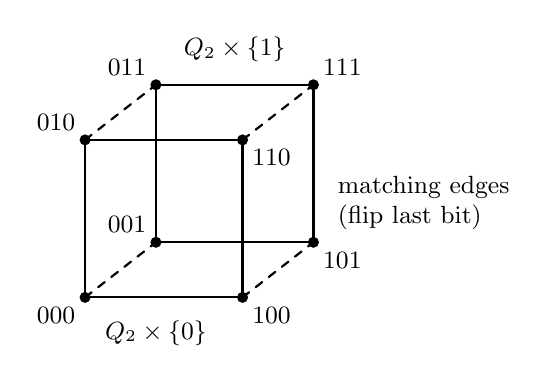
\begin{tikzpicture}[
        scale=1,
        line cap=round,
        line join=round,
        every node/.style={font=\small}
    ]
        % Front square (Q_2 x {0})
        \coordinate (A0) at (0,0);
        \coordinate (B0) at (2,0);
        \coordinate (C0) at (2,2);
        \coordinate (D0) at (0,2);
        % Back square (Q_2 x {1}) shifted
        \coordinate (A1) at (0.9,0.7);
        \coordinate (B1) at (2.9,0.7);
        \coordinate (C1) at (2.9,2.7);
        \coordinate (D1) at (0.9,2.7);
        % Draw Q_2 faces
        \draw[thick] (A0)--(B0)--(C0)--(D0)--cycle;
        \draw[thick] (A1)--(B1)--(C1)--(D1)--cycle;
        % Perfect matching edges
        \draw[dashed, thick] (A0)--(A1);
        \draw[dashed, thick] (B0)--(B1);
        \draw[dashed, thick] (C0)--(C1);
        \draw[dashed, thick] (D0)--(D1);
        % Vertices
        \foreach \p in {A0,B0,C0,D0,A1,B1,C1,D1}{
            \fill (\p) circle (2pt);
        }
        % Labels
        \node[below left]  at (A0) {$000$};
        \node[below right] at (B0) {$100$};
        \node[below right] at (C0) {$110$};
        \node[above left]  at (D0) {$010$};
        \node[above left]  at (A1) {$001$};
        \node[below right] at (B1) {$101$};
        \node[above right] at (C1) {$111$};
        \node[above left]  at (D1) {$011$};
        % Annotations
        \node at (0.9,-0.45) {$Q_2 \times \{0\}$};
        \node at (1.9,3.15) {$Q_2 \times \{1\}$};
        \node[align=left] at (4.3,1.2) {matching edges\\(flip last bit)};
    \end{tikzpicture}
    \caption{%
        The 3-dimensional hypercube $Q_3 \cong Q_2 \square K_2$, visualized as two copies of $Q_2$ with a perfect matching (dashed edges) connecting corresponding vertices that differ in the last bit coordinate.
    }
    \label{fig:ch5_qseq-hypercube}
\end{figure}
\vspace{0.2cm}
\noindent
The following Lemma characterizes balanced partitions of the hypercube satisfying the path-counting symmetry Eq.~\eqref{eq:ch5_qseq-count-condition} which are precisely those obtained by flipping a single coordinate.
\hypercubeflip*

We prove Lemma \ref{lem:ch5_qseq-hypercube-flip} via induction on $n$. 
The following lemma establishes that the two parts must have adjacent vertices.

\begin{lemma}
    \label{lem:ch5_qseq-min-dist}
    Let $A, B \subseteq V(Q_n)$ satisfy the hypotheses of Lemma~\ref{lem:ch5_qseq-hypercube-flip}. 
    Then
    \begin{equation}
        \min\{d(x, y) : x \in A, \, y \in B\} = 1.
    \end{equation}
\end{lemma}

\begin{proof}
    Let $k = \min\{d(x, y) : x \in A, \, y \in B\}$. 
    Assume for contradiction that $k > 1$. 
    Choose $x \in A$ and $y \in B$ with $d(x, y) = k$, and let $\langle x = x_0, x_1, \ldots, x_k = y \rangle$ be a shortest path from $x$ to $y$ in $Q_n$.

    Then $d(x, x_1) = 1$ and $d(x_1, y) = k - 1 < k$. 
    Since $x_1 \in V(Q_n) = A \sqcup B$:
    \begin{itemize}
        \item If $x_1 \in A$, then $d(x_1, y) < k$ with $x_1 \in A$, $y \in B$, contradicting minimality of $k$.
        \item If $x_1 \in B$, then $d(x, x_1) = 1 < k$ with $x \in A$, $x_1 \in B$, again contradicting minimality.
    \end{itemize}
    Hence $k = 1$.
\end{proof}


\begin{proof}[Proof of Lemma~\ref{lem:ch5_qseq-hypercube-flip}]
We proceed by induction on $n$.

\medskip
\noindent\textbf{Base case} ($n=2$):  
The vertex set is $V(Q_2) = \{00, 01, 10, 11\}$. By Lemma~\ref{lem:ch5_qseq-min-dist}, there exist $x \in A$ and $y \in B$ with $d(x,y) = 1$. Without loss of generality, take $x = 00$ and $y = 01$.

Since $|A| = |B| = 2$, the only possible balanced partitions with $00 \in A$ and $01 \in B$ are
\begin{equation}
    A = \{00, 10\}, \; B = \{01, 11\}
    \qquad \text{or} \qquad
    A = \{00, 11\}, \; B = \{01, 10\}.
\end{equation}

In both cases, $B$ is obtained from $A$ by flipping the second coordinate. Thus the claim holds for $n = 2$.

\medskip
\noindent\textbf{Induction step}:  
Assume the claim holds for all dimensions $2 \leq t \leq n$. Consider $Q_{n+1}$.

By Lemma~\ref{lem:ch5_qseq-min-dist}, choose vertices $x \in A$ and $y \in B$ with $d(x,y) = 1$. Let $i \in [n+1]$ be the unique coordinate in which $x$ and $y$ differ.

Using the Cartesian product decomposition $Q_{n+1} \cong Q_n \square K_2$ from Eq.~\eqref{eq:ch5_qseq-cart-prod}, consider an $n$-dimensional sub-cube $H \subseteq Q_{n+1}$ that contains the edge $xy$. 
Within $G$, the induced partition $A \cap V(H)$ and $B \cap V(H)$ still satisfies the counting condition (iii) for all pairs of vertices in $H$. 
By the induction hypothesis applied to $H \cong Q_n$, we get that membership in $A \cap V(H)$ and $B \cap V(H)$ is related by flipping the $i$-th bit.

Now consider a 4-cycle (2-dimensional sub-cube) $x$--$y$--$z$--$w$--$x$ in $Q_{n+1}$ with $z, w \notin V(H)$.
Since $x \in A$ and $y \in B$, applying Eq.~\eqref{eq:ch5_qseq-counting-equality} with $L=2$, we get $z$ and $w$ to lie in opposite partitions. 
Note that $z$ and $w$ differ only in the $i$-th coordinate. 
By the cartesian product structure, there exists another sub-cube $M \cong Q_k$ containing the edge edge $zw$ and is disjoint from $H$. 
Thus, applying the induction hypothesis again, we conclude that the same coordinate $i$ implements the flip globally on all vertices, i.e., for every $v \in V(Q_{n+1})$,
\begin{equation}
    v \in A \quad\Longleftrightarrow\quad v^{(i)} \in B.
\end{equation}

This completes the induction.
\end{proof}

For any pair of vertices $x \in S_0$ and $y \in S_1$ in the Boolean hypercube, consider all vertices $w$ such that a path from $x$ to $y$ via $w$ has total length $L$ (where the path need not be shortest overall, just the sum $d(x,w) + d(w,y) = L$). 
By equating coefficients of powers of $s$ in the polynomial identity we show that, for balanced functions, the number of such intermediate vertices in $S_0$ equals the number in $S_1$, for every choice of $x$, $y$ and $L$.

\begin{theorem}
    \label{thm:ch5_qseq-counting}
    If the PGM (and hence the greedy strategy) is optimal and the function $f$ is balanced, then for all integers $L \in \{0,1,\dots,2n\}$ and for all $x \in S_0$, $y \in S_1$,
    \begin{equation}
        \label{eq:ch5_qseq-counting-equality}
        \bigl|\{\,u \in S_0 : d(x,u) + d(u,y) = L\,\}\bigr| 
        =
        \bigl|\{\,v \in S_1 : d(x,v) + d(v,y) = L\,\}\bigr|
    \end{equation}
    for all but finitely many values of $s \in (0,1)$.
\end{theorem}

\begin{proof}
    From Theorem~\ref{thm:ch5_qseq-gammacomm}, we have $\Gamma_0 \Gamma' = \Gamma' \Gamma_1$. Fix $x \in S_0$ and $y \in S_1$. 
    The $(x,y)$-entries of these matrix products are:
    \begin{equation}
        (\Gamma_0 \Gamma')_{xy} = \sum_{u \in S_0} s^{d(x,u) + d(u,y)},
        \qquad
        (\Gamma' \Gamma_1)_{xy} = \sum_{v \in S_1} s^{d(x,v) + d(v,y)}.
    \end{equation}

    Equality of these expressions as polynomials in $s$ means:
    \begin{equation}
        \sum_{u \in S_0} s^{d(x,u) + d(u,y)} = \sum_{v \in S_1} s^{d(x,v) + d(v,y)}.
    \end{equation}

    We can rewrite each sum by grouping terms according to the total distance $L = d(x,w) + d(w,y)$:
    \begin{equation}
        \sum_{L=0}^{2n} s^L \bigl|\{u \in S_0 : d(x,u) + d(u,y) = L\}\bigr|
        = \sum_{L=0}^{2n} s^L \bigl|\{v \in S_1 : d(x,v) + d(v,y) = L\}\bigr|.
    \end{equation}

    This is a polynomial identity in $s$. 
    For this to hold for all but finitely many values of $s \in (0,1)$, the coefficients of each power $s^L$ on both sides must agree. 
    This gives us Eq.~\eqref{eq:ch5_qseq-counting-equality} for each $L$.
\end{proof}

\subsection{Necessity of the Affine Structure}

We now combine the results from the previous sections to obtain a complete characterization of when the greedy strategy is optimal. 
A crucial element in our proof will be the following Lemma about the Boolean hypercube whose proof can be found in Appendix \ref{app:hypercube}.

\begin{restatable}[Hypercube Flip Characterization]{lemma}{hypercubeflip}
    \label{lem:ch5_qseq-hypercube-flip}
    Let $Q_n$ be the $n$-dimensional hypercube graph, and let $A, B \subseteq V(Q_n)$ be a partition satisfying
    \begin{enumerate}
        \item[(i)] $A \cup B = V(Q_n)$ and $A \cap B = \varnothing$;
        \item[(ii)] $|A| = |B| = 2^{n-1}$ (balanced partition);
        \item[(iii)] for all $L \in \N$ and for all $x \in A$, $y \in B$,
            \begin{equation}
                \label{eq:ch5_qseq-count-condition}
                \bigl|\{\,u \in A: d(x,u) + d(u,y) = L\,\}\bigr|
                =
                \bigl|\{\,v \in B: d(x,v) + d(v,y) = L\,\}\bigr|.
            \end{equation}
    \end{enumerate}
    Then there exists a unique index $i \in [n]$ such that for every $x = (x_1,\dots,x_n) \in \{0,1\}^n$,
    \begin{equation}
        x \in A \quad\Longleftrightarrow\quad x^{(i)} \in B,
    \end{equation}
    where $x^{(i)} = (x_1,\dots,x_{i-1},\overline{x_i},x_{i+1},\dots,x_n)$ denotes the bit-flip of $x$ in the $i$-th coordinate.
\end{restatable}

We start with the following theorem which states that the functions for which the greedy strategy is optimal must necessarily follow a recursive structure.
\begin{theorem}
    \label{thm:ch5_qseq-function-form}
    If the greedy strategy is optimal, then the function is either constant or there exists an index $ i \in [n] $ and a Boolean function $ g : \{0,1\}^{n-1} \to \{0,1\} $ such that
    \begin{equation}
        \label{eq:ch5_qseq-function-xor}
        f(x_1,x_2,\dots,x_n) = g(x_1,\dots,x_{i-1},x_{i+1},\dots,x_n) \oplus x_i 
    \end{equation}
    for all but finitely many values of $s\in (0,1).$
\end{theorem}

\begin{proof}
The case if the function is constant is trivial. 
Assume therefore that the function is not constant.

From Theorem \ref{thm:ch5_qseq-counting}, optimality of the greedy strategy implies that for all $ x \in S_0 $, $ y \in S_1 $, and for all integers $ L $,
\begin{equation}
    \label{eq:ch5_qseq-counting-balance}
    \bigl|\{\,u \in S_0 : d(x,u)+d(u,y)=L\,\}\bigr|
    =
    \bigl|\{\,v \in S_1 : d(x,v)+d(v,y)=L\,\}\bigr|
\end{equation}
for all but finitely many values of the inner product $ s $.

By the hypercube structure of $ \{0,1\}^n $ and Lemma~\ref{lem:ch5_qseq-hypercube-flip}, there exists an index $ i \in [n] $ such that flipping the $i$-th bit maps $S_0$ bijectively onto $S_1$.
Equivalently, for every $x=(x_1,\dots,x_n)\in\{0,1\}^n$,
\begin{equation}
    x \in S_0 \quad\Longleftrightarrow\quad x^{(i)} \in S_1,
\end{equation}
where $x^{(i)}$ denotes the bit-flip of $x$ in the $i$-th coordinate.

Define
\begin{equation}
    g(x_1,\dots,x_{i-1},x_{i+1},\dots,x_n) \coloneqq f(x_1,\dots,x_{i-1},0,x_{i+1},\dots,x_n).
\end{equation}
Then, by construction,
\begin{equation}
    f(x_1,\dots,x_n) = g(x_1,\dots,x_{i-1},x_{i+1},\dots,x_n) \oplus x_i,
\end{equation}
which proves Eq.~\eqref{eq:ch5_qseq-function-xor}.
\end{proof}

The recursive structure revealed in Theorem~\ref{thm:ch5_qseq-function-form} allows us to apply induction to completely characterize optimal functions by proving Theorem \ref{thm:ch5_qseq-necessary}.
\necessity*

\begin{proof}
Since the greedy strategy is globally optimal for evaluating a Boolean function $f$, Theorem~\ref{thm:ch5_qseq-gammacomm} implies that the associated Gram matrices satisfy
\begin{equation}
    \Gamma_0 \Gamma' = \Gamma' \Gamma_1 .
\end{equation}
Therefore, it suffices to show that whenever $\Gamma_0 \Gamma' = \Gamma' \Gamma_1$, the function $f$ must be an affine Boolean function. We prove this statement by induction on the number of variables $n$. 

Without loss of generality, assume that $f(0,\dots,0) = 0$; otherwise, we may replace $f$ by its complement $\overline{f}$, which is equivalent to setting $b_0 = 1$.

\noindent \textbf{Base case}: The case when $n=1$ is trivial. 
Assume therefore that $n=2$. 
By Theorem \ref{thm:ch5_qseq-balanced}, $f$ is either constant or balanced. 
If $f$ is constant, the claim is again trivial. 
If $f$ is balanced with $f(0,0) = 0$, then $|f^{-1}(0)| = 2$. 
The possible choices for $f^{-1}(0) \subseteq \{00, 01, 10, 11\}$ are:
$\{00, 01\}, \{00, 10\},$ and $\{00, 11\}$.

These correspond to the functions:
\begin{equation}
    \begin{aligned}
        f(x_1, x_2) &= x_1, \qquad &\text{(corresponds to $\{00,01\}$)} \\
        f(x_1, x_2) &= x_2, \qquad &\text{(corresponds to $\{00,10\}$)} \\
        f(x_1, x_2) &= x_1 \oplus x_2, \qquad &\text{(corresponds to $\{00,11\}$)}
    \end{aligned}
\end{equation}

All three are affine, confirming the claim for $n = 2$.

\noindent\textbf{Induction step}:  
Assume the statement holds for all positive integers up to $n-1$. Let $f:\{0,1\}^n \to \{0,1\}$ be non-constant, and suppose the greedy strategy is optimal.

By Theorem~\ref{thm:ch5_qseq-function-form}, there exists an index $i \in [n]$ and a function $g:\{0,1\}^{n-1} \to \{0,1\}$ such that
\begin{equation}
    f(x_1,\dots,x_n) = g(x_1,\dots,x_{i-1},x_{i+1},\dots,x_n) \oplus x_i.
\end{equation}

\begin{lemma}
    \label{lem:ch5_qseq-reduced-optimality}
    Let $G_0$ (resp.\ $G_1$) be the Gram matrix of the states corresponding to inputs of $g$ that map to $0$ (resp.\ $1$), and let $G'$ be the cross-Gram matrix. 
    If the greedy strategy is optimal for $f$ and $f$ has the form Eq.~\eqref{eq:ch5_qseq-function-xor}, then $G_0 G' = G' G_1$.
\end{lemma}

\begin{proof}
Since the greedy strategy is optimal, we know from Theorem~\ref{thm:ch5_qseq-gammacomm} that
\begin{equation}
    \label{eq:ch5_qseq-gamma-comm-proof}
    \Gamma_0 \Gamma' = \Gamma' \Gamma_1 .
\end{equation}

Order the elements of $S_0$ by first listing those with $x_i = 0$ and then those with $x_i = 1$.
With respect to this ordering, the Gram matrix $\Gamma_0$ has the block form
\begin{equation}
    \Gamma_0 =
        \begin{pmatrix}
            G_0 & s G' \\
            s G'^{*} & G_1
        \end{pmatrix},
\end{equation}
where $s=\langle\psi_0|\psi_1\rangle$.

Similarly, ordering the elements of $S_1$ first with $x_i=1$ and then with $x_i=0$, we obtain
\begin{equation}
    \Gamma' =
        \begin{pmatrix}
            s G_0 & G' \\
            G'^{*} & s G_1
        \end{pmatrix},
    \qquad
    \Gamma_1 =
        \begin{pmatrix}
            G_0 & s G' \\
            s G'^{*} & G_1
        \end{pmatrix}.
\end{equation}

We now compute both sides of Eq.~\eqref{eq:ch5_qseq-gamma-comm-proof}.
First,
\begin{equation}
    \Gamma_0 \Gamma' =
    \begin{pmatrix}
        s G_0^2 + s G' G'^{*} & G_0 G' + s^2 G' G_1 \\[4pt]
        s^2 G'^{*} G_0 + G_1 G'^{*} & s G'^{*} G' + s G_1^2
    \end{pmatrix}.
\end{equation}
Similarly,
\begin{equation}
\Gamma' \Gamma_1 =
    \begin{pmatrix}
        s G_0^2 + s G' G'^{*} & s^2 G_0 G' + G' G_1 \\[4pt]
        G'^{*} G_0 + s^2 G_1 G'^{*} & s G'^{*} G' + s G_1^2
    \end{pmatrix}.
\end{equation}

Equality of these two matrices implies equality of the off-diagonal blocks, hence
\begin{equation}
    G_0 G' + s^2 G' G_1 = s^2 G_0 G' + G' G_1 .
\end{equation}

Rearranging gives
\begin{equation}
    (1-s^2)\, G_0 G' = (1-s^2)\, G' G_1 .
\end{equation}

Since $s \in (0,1)$, we conclude
\begin{equation}
    G_0 G' = G' G_1 ,
\end{equation}
as claimed. 
\end{proof}

Returning to the main proof: by Lemma~\ref{lem:ch5_qseq-reduced-optimality} and the induction hypothesis, $g$ has the form
\begin{equation}
    g(x_1,\dots,x_{i-1},x_{i+1},\dots,x_n) = b_0 \oplus \bigoplus_{j \neq i} b_j x_j.
\end{equation}

Substituting into Eq.~\eqref{eq:ch5_qseq-function-xor}:
\begin{equation}
    f(x_1,\dots,x_n) = b_0 \oplus \bigoplus_{j \neq i} b_j x_j \oplus x_i = b_0 \oplus \bigoplus_{j=1}^n b_j x_j,
\end{equation}
where we set $b_i = 1$ and $b_j$ for $j \neq i$ come from $g$.

This is precisely the affine form Eq.~\eqref{eq:ch5_qseq-affine}, completing the induction and the proof.
\end{proof}

We briefly outline the essential steps of the proof for the reader's convenience. 
The proof uses an equivalent condition for the optimality of the PGM given by Lemma~\ref{lem:ch5_qseq-pgmopt}. 
This condition is used to establish that if the greedy strategy is optimal for some function, then the Gram matrices of its corresponding Boolean ensemble must satisfy the commutation relation given by Eq.~\eqref{eq:ch5_qseq-gamma-comm} of Theorem~\ref{thm:ch5_qseq-gammacomm}. 
The main consequence of this is Theorem~\ref{thm:ch5_qseq-function-form} which constrains the function to a recursive form given by Eq.~\eqref{eq:ch5_qseq-function-xor}. 
Since we want to characterize the functions for which the greedy strategy is optimal, the proof of Theorem~\ref{thm:ch5_qseq-necessary} starts with Eq.~\eqref{eq:ch5_qseq-gamma-comm} because this is a direct consequence of PGM optimality. 
We then use induction to show that whenever this equation is satisfied, the function is affine. 
Our induction hypothesis is: 
if $f$ is a Boolean function on $(n-1)$-bits for which the greedy strategy is optimal, then Eq.~\eqref{eq:ch5_qseq-gamma-comm} holds which implies $f$ must be affine. 
A key role is played by Lemma~\ref{lem:ch5_qseq-reduced-optimality} which asserts than if the greedy strategy is optimal for $f$ which is an $n$-bit Boolean function satisfying the recursive form Eq.~\eqref{eq:ch5_qseq-function-xor}, then the Gram matrices of the Boolean ensemble of $g$, the $(n-1)$-bit Boolean function that appears in the recursive form of $f$, must satisfy the commutation relation Eq.~\eqref{eq:ch5_qseq-gamma-comm}. 
But by our induction hypothesis, any $(n-1)$-bit Boolean function satisfying Eq.~\eqref{eq:ch5_qseq_gamma-comm} must be affine. 
This implies that $f$ itself must be affine. 

\begin{comment}
\section{Conclusion}
\label{sec:discussion}
We characterized when memoryless measurement strategies suffice for learning Boolean properties of quantum sequences. Given a sequence of $n$ qubits, each in one of two known states $\ket{\psi_0}$ or $\ket{\psi_1}$ having inner product $s \in (0,1)$, the problem is to determine the value of a Boolean function of the (unknown) underlying bit string. We posed this as a state discrimination problem between two mixed states corresponding to the two values of the Boolean function, and studied the minimum-error regime.

We considered a simple greedy strategy which measures each qubit independently to optimally distinguish $\ket{\psi_0}$
from $\ket{\psi_1}$ requiring no quantum or classical memory. We showed that for evaluating affine Boolean functions this strategy is equivalent to the optimal global strategies which utilize quantum memory and joint measurements. We also established the converse of this for all but finitely many values of $s$, i.e., the only functions which can be optimally learned using this greedy strategy are the affine Boolean functions. This means that all other Boolean properties fundamentally require memory for optimal learning.
 
Beyond this characterization, we proved that the greedy strategy always achieves at least the square of the optimal success probability, establishing it as the pretty good measurement for this discrimination problem. This universal guarantee shows that even when not optimal, memoryless strategies remain competitive.
%\ankith{What can we say about the non-affine functions?}
%\tathagata{I have added a reference to the discussion about non-affine functions in the paragraph above section 3.}

Previous works have explored cryptographic primitives in the bounded quantum-storage model \cite{damgaard2008cryptography} and state discrimination with limited quantum memory \cite{ballester2008state}. Since both quantum memory and joint measurements remain technologically challenging \cite{lvovsky2009optical,ma2021one,conlon2023approaching}, characterizing when memoryless strategies suffice is of significant interest. Our results could inform settings such as quantum reading of classical memories \cite{pirandola2011quantum}, and quantum-enhanced pattern recognition \cite{ortolano2023quantum}.

There are several avenues for future research. 
%The first is to study the greedy strategy in unambiguous learning of Boolean properties. 
The first is to study the greedy strategy for learning Boolean properties of quantum sequences for other priors, e.g., unequal, correlated, etc. 
%\alice{We could also maybe mention as a future direction generalizing fully memoryless strategies to account for unequal priors.} 
%\snote{I commented out the unambiguous direction and added in Alice's suggestion.}
The second is to introduce limited classical memory to allow some degree of adaptation. It is of interest to investigate which other classes of Boolean functions can be optimally learned using adaptive local strategies. 
%One can also introduce quantum memory and investigate which classes of functions necessarily require joint measurements for their optimal evaluation. 
Finally, studying online or streaming strategies where qubits arrive sequentially and the Boolean function value is continuously updated as the sequence grows, is another direction for future research. 
\end{comment}

%------------------------------------------------------------------------------%
\subsection*{Software} 
%------------------------------------------------------------------------------%

Companion software for computing optimal discrimination probabilities,
including the semidefinite programs used in this work, is available in the
\texttt{toqito} quantum information package~\cite{russo2021toqito}.

\begin{comment}
\subsection*{Acknowledgements}
We thank Gary Au for helpful discussions on some of our combinatorial arguments.  
J.S. and A.Z~are funded in part by the Commonwealth of Virginia's Commonwealth Cyber Initiative (CCI) under grant number 469351.
T.G.~acknowledges the Indian Statistical Institute, Kolkata for support during the early stages of this work.
T.G.~acknowledges financial support from the ANRF National Post-Doctoral Fellowship (NPDF) under File No.~PDF/2025/005147.
\end{comment}

%\bibliographystyle{unsrt}
%\bibliography{bib} 

%\appendix
%==============================================================================
\begin{comment}
\section{The Pretty Good Measurement}\label{app:pgm}

The \emph{pretty good measurement} (PGM), introduced by Hausladen and Wootters~\cite{hausladen1994pretty} and further analyzed by Barnum and Knill~\cite{barnum2002reversing}, provides a computationally tractable measurement strategy for quantum state discrimination. Given an ensemble $\{(p_i, \rho_i)\}_{i=1}^n$, the PGM defined by the measurement operators
\begin{equation}
\label{eq:pgm-operators}
    M_i^{\text{PGM}} = \rho_{\text{avg}}^{-1/2} (p_i \rho_i) \rho_{\text{avg}}^{-1/2},
\end{equation}
where $\rho_{\text{avg}} = \sum_{i=1}^n p_i \rho_i$ and $\rho_{\text{avg}}^{-1/2}$ denotes its Moore-Penrose pseudo-inverse. These operators form a valid POVM.%: they are positive semidefinite and satisfy $\sum_{i=1}^n M_i^{\text{PGM}} = \I$.

Barnum and Knill~\cite{barnum2002reversing} gave the following bound on the performance of the PGM.
%The performance of the PGM is characterized by the following inequality due to Barnum and Knill~\cite{barnum2002reversing}:

\begin{theorem}%[Barnum-Knill Inequality]
\label{thm:barnum-knill}
Let $P_{\text{opt}}$ denote the optimal success probability and $P_{\text{PGM}}$ denote the success probability achieved by the pretty good measurement for discriminating an ensemble $\{(p_i, \rho_i)\}_{i=1}^n$. Then
\begin{equation}
    P_{\text{opt}}^2 \leq P_{\text{PGM}} \leq P_{\text{opt}}.
\end{equation}
\end{theorem}

This bound ensures that the PGM always achieves a success probability at least as large as the square of the optimal probability, guaranteeing near-optimal performance. Moreover, in many cases of interest, the PGM is exactly optimal \cite{mochon2006family,dalla2015optimality,eldar2001quantum}.

%For our problem of Boolean function evaluation, we will establish in Theorem~\ref{thm:pgm-local} that the PGM operators defined by Eq.~\eqref{eq:pgm-operators} decompose exactly as the measurement operators of the fixed greedy strategy. This remarkable structural property will be central to our characterization of when local measurements suffice.
\end{comment}
%===============================================================================





%-----------------------------------------------------------------------------%
\section{Greedy Strategy Performance for Non-Affine Functions} \label{app:non-affine-examples}

In this section, we examine two important non-affine functions: the AND function and the majority function. 
For these functions, the greedy strategy is suboptimal, but understanding the gap between greedy and global performance provides insight into when adaptive or joint measurements offer practical advantages.

\subsection{The AND Function}

The AND function on $n$ bits is defined by
\begin{equation}
    f_{\text{AND}}(x_1,\dots,x_n) = x_1 \wedge x_2 \wedge \cdots \wedge x_n = 
        \begin{cases}
            1 & \text{if } x_i = 1 \text{ for all } i, \\
            0 & \text{otherwise}.
        \end{cases}
\end{equation}

This function is highly unbalanced: $S_1 = \{11\ldots1\}$ contains only the all-ones string, while $S_0$ contains all other $2^n - 1$ strings.

\subsubsection{Greedy Success Probability}

For the greedy strategy, we measure each qubit independently using the optimal single-qubit measurement, which succeeds with probability $p = \frac{1}{2} + \frac{1}{4} \left\| \op{\psi_0} - \op{\psi_1} \right\|_1$ when distinguishing $\ket{\psi_0}$ from $\ket{\psi_1}$ with equal priors.

The greedy strategy fails in evaluating $f_{\text{AND}}$ correctly if and only if:
\begin{itemize}
    \item When $x = 11\ldots1$: we guess $y \neq 11\ldots1$, which occurs with probability $1-p^n$.
    \item When $x \neq 11\ldots1$: we guess any $y = 11\ldots1$, which occurs with probability $1 - p^n$.
\end{itemize}

The greedy success probability is therefore:
\begin{equation}
    \begin{aligned}
        P(n,\AND,s,\greedy) &= 1-\frac{1}{2^{n-1}} \cdot (1-p^n).
    \end{aligned}
\end{equation}


\begin{figure}[t]
    \centering
    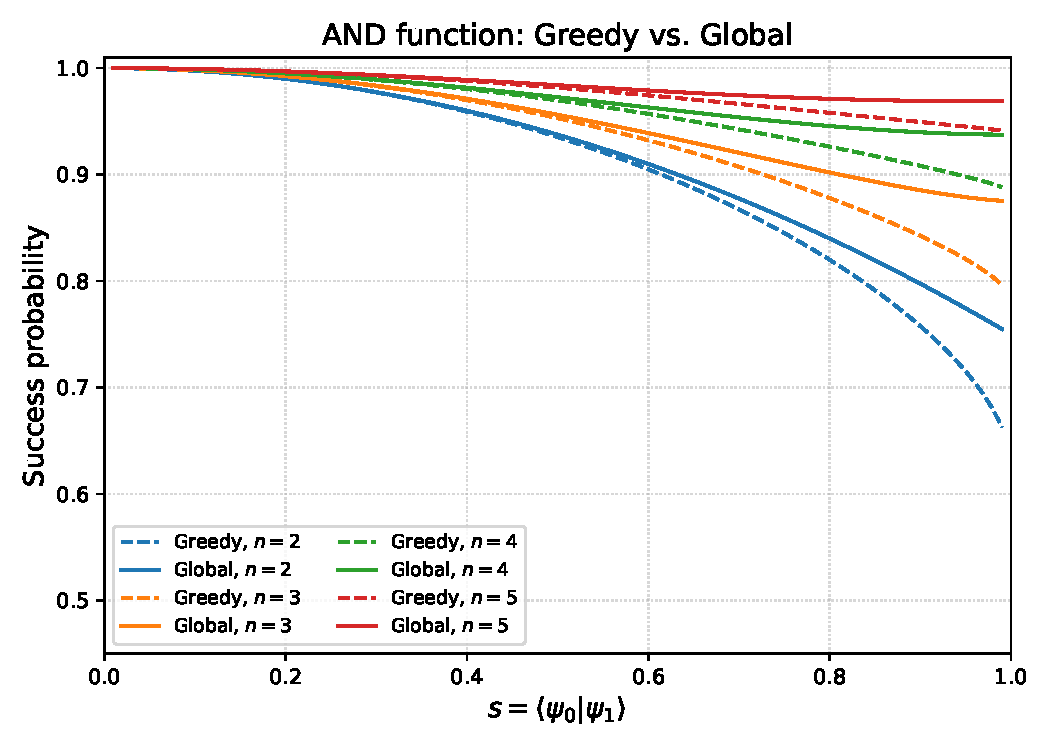
\includegraphics[scale=0.75]{figs/ch5_qseq/greedy_vs_global_AND.pdf}
    \caption{Local vs.~global success probabilities for the AND function. As $n$ increases, both strategies approach perfect success exponentially fast, with the gap diminishing rapidly.}
    \label{fig:and-comparison}
\end{figure}




\subsubsection{Asymptotic Behavior}

As $n \to \infty$ with $p \in (1/2,1)$ fixed (corresponding to fixed non-orthogonal states $\ket{\psi_0}$ and $\ket{\psi_1}$):
\begin{equation}
    P(n,\AND,s,\greedy) = 1 - \frac{(1 - p)^n}{2^n} \to 1,
\end{equation}
since both $(1-p)^n \to 0$ and $1/2^n \to 0$ exponentially fast.

This limiting behavior is intuitive: 
with overwhelming probability $(2^n-1)/2^n \to 1$, the input contains at least one zero. 
The probability of accidentally guessing all ones when the input is not all ones is $p^n$, which vanishes exponentially. 
Thus, the greedy strategy succeeds with probability approaching 1. 
The global optimal strategy achieves slightly better performance by leveraging correlations across qubits, but this advantage becomes negligible as $n$ increases. 
For large $n$, the extreme imbalance of the AND function dominates, and both strategies approach perfect success.

\subsection{The Majority Function}

For odd $n = 2k+1$, the majority function is defined by
\begin{equation}
    f_{\text{maj}}(x_1,\dots,x_{2k+1}) = 
        \begin{cases}
            1 & \text{if } \sum_{i=1}^{2k+1} x_i > k, \\
            0 & \text{if } \sum_{i=1}^{2k+1} x_i \leq k.
        \end{cases}
\end{equation}

Unlike the AND function, majority is balanced: $|S_0| = |S_1| = 2^{2k}$.

\subsubsection{Greedy Success Probability}

We now compute the greedy success probability for the majority function rigorously. 
The greedy strategy measures each qubit independently with the optimal single-qubit measurement, which correctly identifies the bit value with probability $p$ and incorrectly identifies it with probability $1-p$.

Given an input string $x$ with Hamming weight $w(x) = j$ (i.e., $j$ ones and $2k+1-j$ zeros), the measurement produces an output string $y$ whose Hamming weight $w(y)$ is a random variable. 
We can decompose $w(y)$ as:
\begin{equation}
w(y) = Y_1 + Y_2,
\end{equation}
where:
\begin{itemize}
    \item $Y_1$ is the number of ones in $y$ that came from ones in $x$ (correctly identified ones), with $Y_1 \sim \text{Binomial}(j, p)$;
    \item $Y_2$ is the number of ones in $y$ that came from zeros in $x$ (incorrectly flipped zeros), with $Y_2 \sim \text{Binomial}(2k+1-j, 1-p)$.
\end{itemize}

Since different qubits are measured independently, $Y_1$ and $Y_2$ are independent random variables.

The greedy strategy succeeds when $f_{\text{maj}}(x) = f_{\text{maj}}(y)$, which occurs when:
\begin{itemize}
    \item If $j \leq k$ (so $f(x) = 0$): we need $w(y) \leq k$, i.e., $Y_1 + Y_2 \leq k$.
    \item If $j > k$ (so $f(x) = 1$): we need $w(y) > k$, i.e., $Y_1 + Y_2 > k$.
\end{itemize}

Let $\gamma_j$ denote the conditional success probability given that $w(x) = j$. For $j \leq k$:
\begin{equation}
    \gamma_j = P(Y_1 + Y_2 \leq k) = \sum_{a=0}^{j} \sum_{b=0}^{\min(2k+1-j, k-a)} \binom{j}{a} p^a (1-p)^{j-a} \binom{2k+1-j}{b} (1-p)^b p^{2k+1-j-b}.
\end{equation}

For $j > k$ (equivalently, $j \geq k+1$):
\begin{equation}
    \gamma_j = P(Y_1 + Y_2 > k) = \sum_{a=0}^{j} \sum_{b=\max(0,k+1-a)}^{2k+1-j} \binom{j}{a} p^a (1-p)^{j-a} \binom{2k+1-j}{b} (1-p)^b p^{2k+1-j-b}.
\end{equation}

By symmetry of the majority function, we have $\gamma_j = \gamma_{2k+1-j}$ for all $j$. 
To see this, note that if we flip all bits in both $x$ and $y$, the majority value also flips, and the distribution of measurement outcomes remains the same (with the roles of 0 and 1 interchanged). 
Therefore, the conditional success probability for $j$ ones is the same as for $j$ zeros (i.e., $2k+1-j$ ones).

The greedy success probability is:
\begin{equation}
    \begin{aligned}
        P(n=2k+1,\MAJ,s,\greedy) &= \sum_{j=0}^{2k+1} \frac{1}{2^{2k+1}} \binom{2k+1}{j} \gamma_j \\
        &= 2\sum_{j=0}^{k} \frac{1}{2^{2k+1}} \binom{2k+1}{j} \gamma_j \\
        &= \sum_{j=0}^{k} \frac{1}{2^{n-1}} \binom{2k+1}{j} \gamma_j,
    \end{aligned}
\end{equation}
where we used the symmetry $\gamma_j = \gamma_{2k+1-j}$ to combine terms.

\begin{figure}[t]
\centering
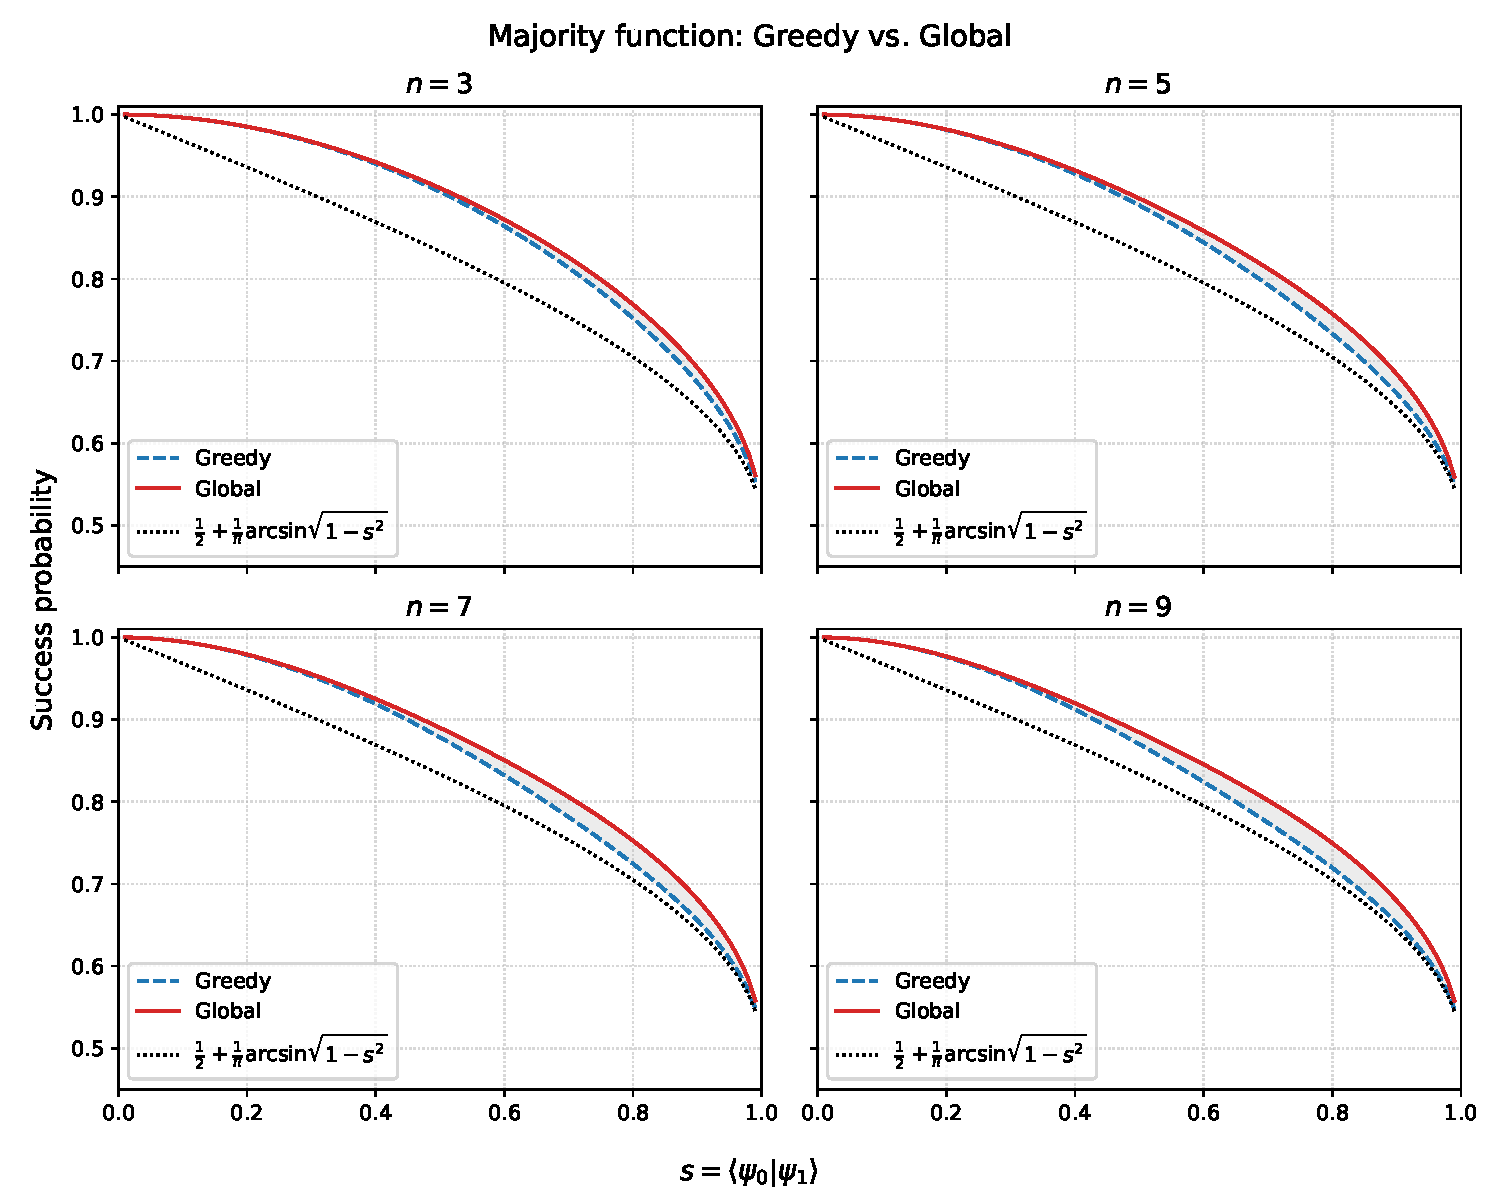
\includegraphics[scale=0.6]{figs/ch5_qseq/greedy_vs_global_MAJ_separate.pdf}
\caption{Local vs.~global success probabilities for the majority function}
\label{fig:maj-comparison}
\end{figure}


\subsubsection{Asymptotic Behavior}

The asymptotic behavior of the majority function is governed by its noise sensitivity. 
Unlike the AND function, the failure probability for majority does not vanish as $n \to \infty$.

To analyze this, we relate our setting to the noise sensitivity framework. 
When we measure each qubit with the optimal single-qubit measurement, we correctly identify each bit with probability $p=\frac{1}{2}(1+\sqrt{1-s^2})$ and incorrectly with probability $\epsilon := 1-p$. 
This is equivalent to applying independent random noise to each bit with noise rate $\epsilon$.

The noise sensitivity of the majority function has been precisely characterized \cite{mossel2003noise}. 
For the majority function on $n = 2k+1$ bits with noise parameter $\epsilon$, the probability that the function value changes (i.e., the failure probability) is given by:
\begin{equation}
    P_{\text{fail}}^{\text{maj}} = \frac{1}{2}- \frac{1}{\pi}\arcsin({1-2\epsilon}) + O\left(\frac{1}{\sqrt{n\epsilon}}\right).
\end{equation}

In the limit as $n \to \infty$ with small $\epsilon$, this approaches:
\begin{equation}
    P_{\text{fail}}^{\text{maj}} \to \frac{2}{\pi}(\sqrt{\epsilon}) = \frac{2}{\pi}(\sqrt{1-p}).
\end{equation}

Therefore, the local success probability approaches:
\begin{equation}
    P(n,\MAJ,s,\greedy) \to\frac{1}{2}+ \frac{1}{\pi}\arcsin({\sqrt{1-s^2}}) \text{ as } n \to \infty.
\end{equation}

This limiting value is strictly less than 1 for any $p < 1$ (i.e., for non-orthogonal states). 




\subsection{Comparison and Discussion}

The contrasting behaviors of the AND and majority functions illustrate two distinct regimes:

\paragraph{Highly unbalanced functions (AND):} 
When $|S_0| \gg |S_1|$ or vice versa, the greedy strategy performs nearly optimally for large $n$ because the overwhelming size of one pre-image dominates the success probability. 
Both local and global strategies converge to perfect success exponentially fast as $n \to \infty$, and the advantage from joint measurements becomes negligible in this regime.

\paragraph{Balanced non-affine functions (majority):} 
For balanced functions that are not affine, the situation is fundamentally different. 
The majority function's noise sensitivity ensures that the greedy strategy converges to a limiting success probability strictly bounded away from 1. 
Specifically, $P(n,\MAJ,s,\greedy) \to 1 - \frac{2}{\pi}\arcsin(\sqrt{1-p})$ as $n \to \infty$, which remains bounded below 1 for any non-orthogonal states ($p < 1$), while the global optimal strategy achieves better performance. 
This gap between local and global strategies persists even asymptotically, demonstrating a persistent advantage of joint measurements that does not vanish as the problem size increases.

These examples confirm that our characterization theorem captures a fundamental dichotomy: affine functions are the unique class where local measurements are always optimal, while all other functions require joint measurements. 
Crucially, the practical significance of this advantage is intimately tied to the function's noise sensitivity. 
Low noise sensitivity functions (like AND for large $n$) exhibit vanishing advantage from joint measurements, while high noise sensitivity functions (like majority) maintain substantial joint-measurement-advantage even for arbitrarily large input dimensions. 
This connection between noise sensitivity and joint-measurement-advantage suggests deeper structural relationships between classical Boolean function complexity and quantum information-theoretic resources.